\documentclass[11pt,a4paper]{article}

\usepackage[a4paper,top=2.4cm,bottom=2.4cm,left=2.8cm,right=2.8cm]{geometry}

\usepackage{fontspec}

\usepackage[english]{babel}

\usepackage{amsmath,amssymb}

\usepackage{booktabs}

\usepackage{array}

\usepackage{tabularx}

\usepackage{graphicx}

\graphicspath{{figures/}}

\usepackage{subcaption}

\usepackage{microtype}

\usepackage{siunitx}

\usepackage{enumitem}

\usepackage{cite}

\usepackage{hyperref}

\hypersetup{
  colorlinks=true,
  linkcolor=blue,
  citecolor=blue,
  urlcolor=blue,
  pdftitle={From Clinical Characteristics to Surgical Pathology: OSCC Recurrence},
  pdfauthor={Mahdi Boughrous et al.}
}

\setlist[itemize]{leftmargin=1.5em,noitemsep,topsep=2pt}

\setlist[enumerate]{leftmargin=1.7em,noitemsep,topsep=2pt}

\newcommand{\ROC}{\text{ROC-AUC}}

\newcommand{\AUPRC}{\text{AUPRC}}

\newcommand{\Brier}{\text{Brier}}

\newcommand{\OR}{\text{OR}}

\newcommand{\aOR}{\text{aOR}}

\newcommand{\CI}{\text{CI}}

\newcommand{\RF}{\text{RF}}

\newcommand{\LR}{\text{LR}}

\emergencystretch=1em
\AtBeginDocument{\normalsize}

\begin{document}

% --- PAGE DE GARDE ---

\thispagestyle{empty}

\begin{titlepage}

\centering

\vspace*{0.7cm}

\begin{minipage}{0.25\textwidth}

\centering


\includegraphics[width=3.2cm]{logo.png}

\end{minipage}\\[0.8cm]

{\fontsize{20}{24}\selectfont\bfseries Mini-Project Report}\\[0.4cm]

{\fontsize{16}{19}\selectfont From Clinical Characteristics to Surgical Pathology: Statistical and Machine-Learning Analysis of Recurrence Risk\\
in Oral Squamous Cell Carcinoma}\\[0.8cm]

\begin{minipage}{0.85\textwidth}

\centering

\textbf{Supervised by:} \\[0.2cm]

Prof. Aziz OUHINOU \\[0.1cm]

Prof. Hicham Moussa

\end{minipage}\\[1.0cm]

% Membres du groupe

\begin{tabular}{|l|l|l|}

\hline

\textbf{Name} & \textbf{Specialization} & \textbf{Laboratory} \\

\hline

Mohamed Taha Benhassoun & Biology & -- \\

Mustapha Amarzoug & Organic Chemistry & 3BIO \\

Yasmine Elasri & Mathematics & Lab. MPA \\

Mahdi Boughrous & Artificial Intelligence & Lab. TIAD \\

Yassin Oulhammous & Artificial Intelligence & Lab. TIAD \\

\hline

\end{tabular}\\[1.2cm]

% Mots-clés

\begin{minipage}{0.85\textwidth}

\textbf{Keywords:} OSCC, recurrence, logistic regression, random forest, machine learning, pathology, calibration, bootstrap, Python.

\end{minipage}\\[1.2cm]

\vfill

\end{titlepage}

% --- FIN PAGE DE GARDE ---

\newpage

\setcounter{page}{1}

\begin{center}

\vspace*{-2em}

\end{center}

\begin{abstract}
\normalsize Recurrence after treatment is an important prognostic problem in oral squamous cell carcinoma (OSCC). This study asks two related questions: which structured clinical characteristics are associated with recurrence, and how much additional predictive signal is contained in pathological characteristics obtained from surgical specimens? The Multi-OSCC cohort included 1,325 patients and 275 recurrence events (20.75\%). Because the pathology variables are obtained from surgical specimens and the outcome is defined as two-year recurrence after surgery, the study does not claim a single pre-treatment prediction time point. Instead, it compares clinical-only, pathology-only, and combined information using non-parametric tests, effect sizes, multivariable logistic regression, Logistic Regression (LR), and Random Forest (RF).

Tumor Differentiation (TD) remained associated with recurrence after adjustment (adjusted odds ratio, \aOR{} = 1.387, 95\% \CI{}: 1.125--1.711; $p=0.0022$). No association was detected for smoking, alcohol use, betel-nut use, or measured systemic comorbidities. On the held-out test set ($n=200$; 49 events), Pathology RF had the highest observed \ROC{} of 0.627 (bootstrap 95\% \CI{}: 0.528--0.724), whereas Combined LR had the highest observed \AUPRC{} of 0.429. Clinical-only models achieved \ROC{} values of 0.534--0.537. At a validation-selected threshold of 0.453, Pathology RF detected 41 of 49 recurrences (recall = 0.837), but specificity was 0.311. All models had \Brier{} scores above the prevalence-only benchmark, and calibration intercepts indicated systematic upward displacement of predicted recurrence probabilities. The results illustrate how statistical association analysis and machine learning answer different questions, while moderate discrimination, uncertainty, and the temporal availability of pathology variables limit direct clinical interpretation and support external validation.
\end{abstract}

\section{Introduction}

Oral cavity cancer is a substantial global health burden, with approximately 377,000 incident cases and 177,000 deaths estimated worldwide in 2020 \cite{sung_global_2021}. Oral squamous cell carcinoma (OSCC) is the predominant malignancy of the oral cavity. Despite treatment, recurrence remains an important clinical outcome because it influences subsequent surveillance and management.

The central idea of this study is simple: not all information about a patient is available at the same stage of care. Clinical characteristics may describe the patient and tumor before or around initial treatment, whereas pathological characteristics such as tumor differentiation and invasion are obtained from the resected specimen. The statistical question is therefore not only whether a variable is associated with recurrence, but also whether adding information that becomes available later changes out-of-sample predictive performance.

Tobacco, alcohol, and betel-quid exposure are established etiologic factors for oral carcinogenesis \cite{sung_global_2021}. However, factors associated with carcinogenesis need not be equally informative for recurrence after treatment. Histopathological markers may instead capture aspects of tumor phenotype related to differentiation, invasion, and aggressive behaviour \cite{almangush_staging_2020}.

This study therefore evaluates the same cohort from two complementary perspectives. First, statistical inference asks which clinical and pathological characteristics are associated with recurrence after accounting for other measured variables. Second, machine learning asks whether these structured variables contain reproducible predictive signal on unseen patients. We address three questions:
\begin{enumerate}
    \item \textbf{Clinical question:} Which patient-level clinical characteristics are associated with recurrence?
    \item \textbf{Pathological question:} Which surgical-pathology characteristics remain associated with recurrence after adjustment for clinical characteristics?
    \item \textbf{Predictive question:} How do discrimination, precision--recall performance, calibration, and threshold behaviour change when clinical variables, pathology variables, or both are used?
\end{enumerate}
The comparison with richer whole-slide image representations is treated as context rather than as a direct performance benchmark \cite{guan2026multi}.

\paragraph{Study logic in plain language.} The study follows one simple chain: first ask whether patient and tumor characteristics are associated with recurrence; then ask whether pathology obtained from the resected tumor contains additional recurrence-related information; finally ask whether this information is useful for prediction on patients not used during model development. This distinction matters because statistical association, predictive discrimination, and clinical usefulness are different properties.

\[
\text{Clinical characteristics} \;\longrightarrow\; \text{Surgical pathology} \;\longrightarrow\; \text{Two-year recurrence after surgery}
\]

\section{Materials and Methods}

\subsection{Cohort and Outcome}

The Multi-OSCC benchmark dataset comprised 1,325 OSCC patients \cite{guan2026multi}. The dataset paper describes a retrospective cohort of surgically treated patients and defines the prognostic REC task as two-year tumor recurrence after surgery \cite{guan2026multi}. Clinical and pathology records were linked using patient identifiers. The outcome used here was binary recurrence:

\begin{equation}
P(\mathrm{REC}=1)=\frac{275}{1325}=20.75\%.
\end{equation}

The non-recurrence group contained 1,050 patients (79.25\%). Importantly, this is not a single pre-treatment prediction problem. TD, TI, CE, and PI are pathology variables obtained from surgical specimens, while REC refers to recurrence after surgery \cite{guan2026multi}. We therefore treat the analysis as a comparison of information available at different stages of care. To reduce obvious target leakage, variables recorded after treatment or after recurrence manifestation were excluded, including surgical margins, flap reconstruction, postoperative tracheostomy, adjuvant radiotherapy, chemotherapy, recurrence-free interval, and follow-up duration. No claim of pre-treatment applicability is made for models containing TD, TI, CE, or PI.

\begin{center}
\small
\begin{tabularx}{0.96\linewidth}{@{}>{\raggedright\arraybackslash}l>{\raggedright\arraybackslash}X>{\raggedright\arraybackslash}X@{}}
\toprule
\textbf{Information stage} & \textbf{Examples used here} & \textbf{Interpretation} \\
\midrule
Clinical characteristics & Age, BMI, exposures, comorbidities, primary tumor site & Baseline/clinical information evaluated as an early information set; exact prospective availability of every field was not assumed. \\
Surgical pathology & TD, TI, CE, PI & Tumor characteristics obtained from the surgical specimen; these variables are not treated as pre-treatment predictors. \\
Outcome & REC & Two-year recurrence after surgery. \\
\bottomrule
\end{tabularx}
\end{center}

Missing values encoded as \texttt{/} were converted to missing values. Age was missing for 8 patients (0.6\%), BMI for 45 (3.4\%), and HPV status for 297 (22.4\%). HPV was excluded because of substantial missingness. Continuous predictors were median-imputed for machine-learning analyses; logistic regression used complete cases.

\subsection{Data Partitioning and Models}

The official patient-level partition (\texttt{split\_seed=2024.json}) was used: training ($n=925$), validation ($n=200$), and held-out test ($n=200$). No patient appeared in more than one partition. Preprocessing was fit only on the training partition.

Three feature configurations were evaluated:

\begin{itemize}

    \item \textbf{Clinical-only:} age, BMI, gender, smoking, alcohol, betel-nut use, ASA grade, diabetes, cardiovascular disease, medicated hypertension, and primary surgical site.

    \item \textbf{Pathology-only:} tumor differentiation (TD), tumor invasion (TI), cancer embolus (CE), and perineural invasion (PI).

    \item \textbf{Combined:} the union of Clinical-only and Pathology-only variables.

\end{itemize}

We fitted $L_2$-regularized LR and RF classifiers. Both LR and RF used balanced class weights to account for the 20.75\% recurrence prevalence. This reweighting inflates predicted recurrence probabilities relative to the true prevalence and is the likely cause of the upward calibration shift reported in Section~\ref{sec:calibration}; it affects Brier score and threshold-based metrics more than ROC-AUC or AUPRC. RF used 200 trees, maximum depth four, and balanced class weights. Continuous predictors were standardized after median imputation; categorical variables were one-hot encoded. The transformed matrices contained 27, 9, and 36 columns for Clinical-only, Pathology-only, and Combined models, respectively.

\subsection{Statistical Analysis}

The statistical and predictive analyses answer different questions. Association tests describe whether variables differ between recurrence groups; logistic regression estimates adjusted associations; machine-learning evaluation measures out-of-sample predictive performance. Because recurrence prevalence was 20.75\%, accuracy alone could be misleading, so we report \ROC{} and \AUPRC{} together with calibration and threshold-dependent measures.

Continuous variables were compared with Mann--Whitney U tests and median differences. Categorical variables were compared using Pearson chi-square tests with Cram\'er's $V$ effect sizes. Univariate and multivariable logistic regression models were fitted on complete cases ($n=1,317$). Primary surgical site was excluded from the adjusted parametric model because sparse events in minority sites generated quasi-complete separation, but it was retained in machine-learning models.

Performance on the held-out test cohort was assessed with \ROC{}, \AUPRC{}, F1 score, recall, specificity, and \Brier{} score. Bootstrap confidence intervals used 1,000 resamples of held-out predictions. A validation-selected threshold maximizing F1 score was applied unchanged to the test cohort. Calibration intercepts and slopes were estimated using logistic calibration models.

\section{Results}

\subsection{Baseline Associations}

Patients with recurrence were younger than those without recurrence (median 56.0 versus 59.0 years; $p=0.015$) and had lower BMI (21.8 versus 22.5 kg/m$^2$; $p=0.012$). Smoking, alcohol use, and betel-nut use showed no significant unadjusted association with recurrence.

Pathology variables showed stronger unadjusted associations. TD, TI, CE, and PI were associated with recurrence in contingency analyses. Primary surgery site was also associated with recurrence; gingiva and jaw tumors had a recurrence proportion of 28.0\%, compared with 18.6\% for tongue tumors.

\begin{table}[htbp]

\centering

\small

\setlength{\tabcolsep}{2.5pt}

\caption{Selected Baseline Characteristics by Recurrence Status ($N=1,325$).}

\label{tab:baseline}

\begin{tabular*}{\linewidth}{@{\extracolsep{\fill}}lccccc@{}}

\toprule

\textbf{Variable} & \textbf{Overall} & \textbf{REC=0} & \textbf{REC=1} & \textbf{Effect} & \textbf{$p$} \\

\midrule

Age, median [IQR] & 58 [50--68] & 59 [50--68] & 56 [47--65] & $\Delta=-3$ & 0.015 \\

BMI, median [IQR] & 22.4 [20.1--25.1] & 22.5 [20.2--25.3] & 21.8 [19.8--24.5] & $\Delta=-0.7$ & 0.012 \\

Smoking history & 518 (39.1\%) & 416 (40.0\%) & 102 (37.1\%) & $V=0.019$ & 0.487 \\

Alcohol history & 304 (22.9\%) & 243 (23.3\%) & 61 (22.2\%) & $V=0.007$ & 0.797 \\

Betel-nut history & 85 (6.4\%) & 66 (6.3\%) & 19 (6.9\%) & $V=0.007$ & 0.812 \\

Tumor differentiation & & & & $V=0.111$ & $<0.001$ \\

\quad Well & 450 (34.0\%) & 377 (35.9\%) & 73 (26.5\%) & & \\

\quad Moderate & 692 (52.2\%) & 546 (52.0\%) & 146 (53.1\%) & & \\

\quad Poor & 183 (13.8\%) & 127 (12.1\%) & 56 (20.4\%) & & \\

Tumor invasion & 618 (46.6\%) & 470 (44.8\%) & 148 (53.8\%) & $V=0.072$ & 0.009 \\

Cancer embolus & 112 (8.5\%) & 79 (7.5\%) & 33 (12.0\%) & $V=0.062$ & 0.024 \\

Perineural invasion & 244 (18.4\%) & 176 (16.8\%) & 68 (24.7\%) & $V=0.081$ & 0.003 \\

\bottomrule

\end{tabular*}

\vspace{0.1cm}

\parbox{\linewidth}{\footnotesize \textit{Notes:} $\Delta$ is the recurrence minus non-recurrence median. $V$ is Cram\'er's $V$.}

\end{table}

\subsection{Adjusted Associations}

In univariate models, TD, TI, CE, and PI were associated with recurrence. After adjustment, TD remained associated with recurrence, whereas TI, CE, and PI attenuated and their confidence intervals included the null. Age had a small inverse adjusted association with recurrence.

\begin{table}[htbp]

\centering

\small

\caption{Multivariable Logistic Regression for OSCC Recurrence ($n=1,317$).}

\label{tab:mlr}

\begin{tabular*}{\linewidth}{@{\extracolsep{\fill}}lccc@{}}

\toprule

\textbf{Predictor} & \textbf{Adjusted OR} & \textbf{95\% CI} & \textbf{$p$-value} \\

\midrule

Age, per year & 0.988 & [0.977, 0.999] & 0.0306 \\

Female versus male & 0.981 & [0.700, 1.376] & 0.9136 \\

Smoking history & 0.822 & [0.568, 1.191] & 0.3012 \\

Alcohol history & 0.940 & [0.639, 1.384] & 0.7545 \\

Betel-nut history & 1.119 & [0.631, 1.983] & 0.7013 \\

ASA physical status & 1.003 & [0.831, 1.210] & 0.9764 \\

Diabetes mellitus & 1.363 & [0.918, 2.022] & 0.1244 \\

Cardiovascular disease & 1.018 & [0.616, 1.683] & 0.9438 \\

Tumor differentiation & \textbf{1.387} & \textbf{[1.125, 1.711]} & \textbf{0.0022} \\

Tumor invasion & 1.262 & [0.919, 1.732] & 0.1499 \\

Cancer embolus & 1.413 & [0.904, 2.211] & 0.1294 \\

Perineural invasion & 1.198 & [0.820, 1.749] & 0.3501 \\

\bottomrule

\end{tabular*}

\end{table}

\begin{figure}[htbp]

\centering

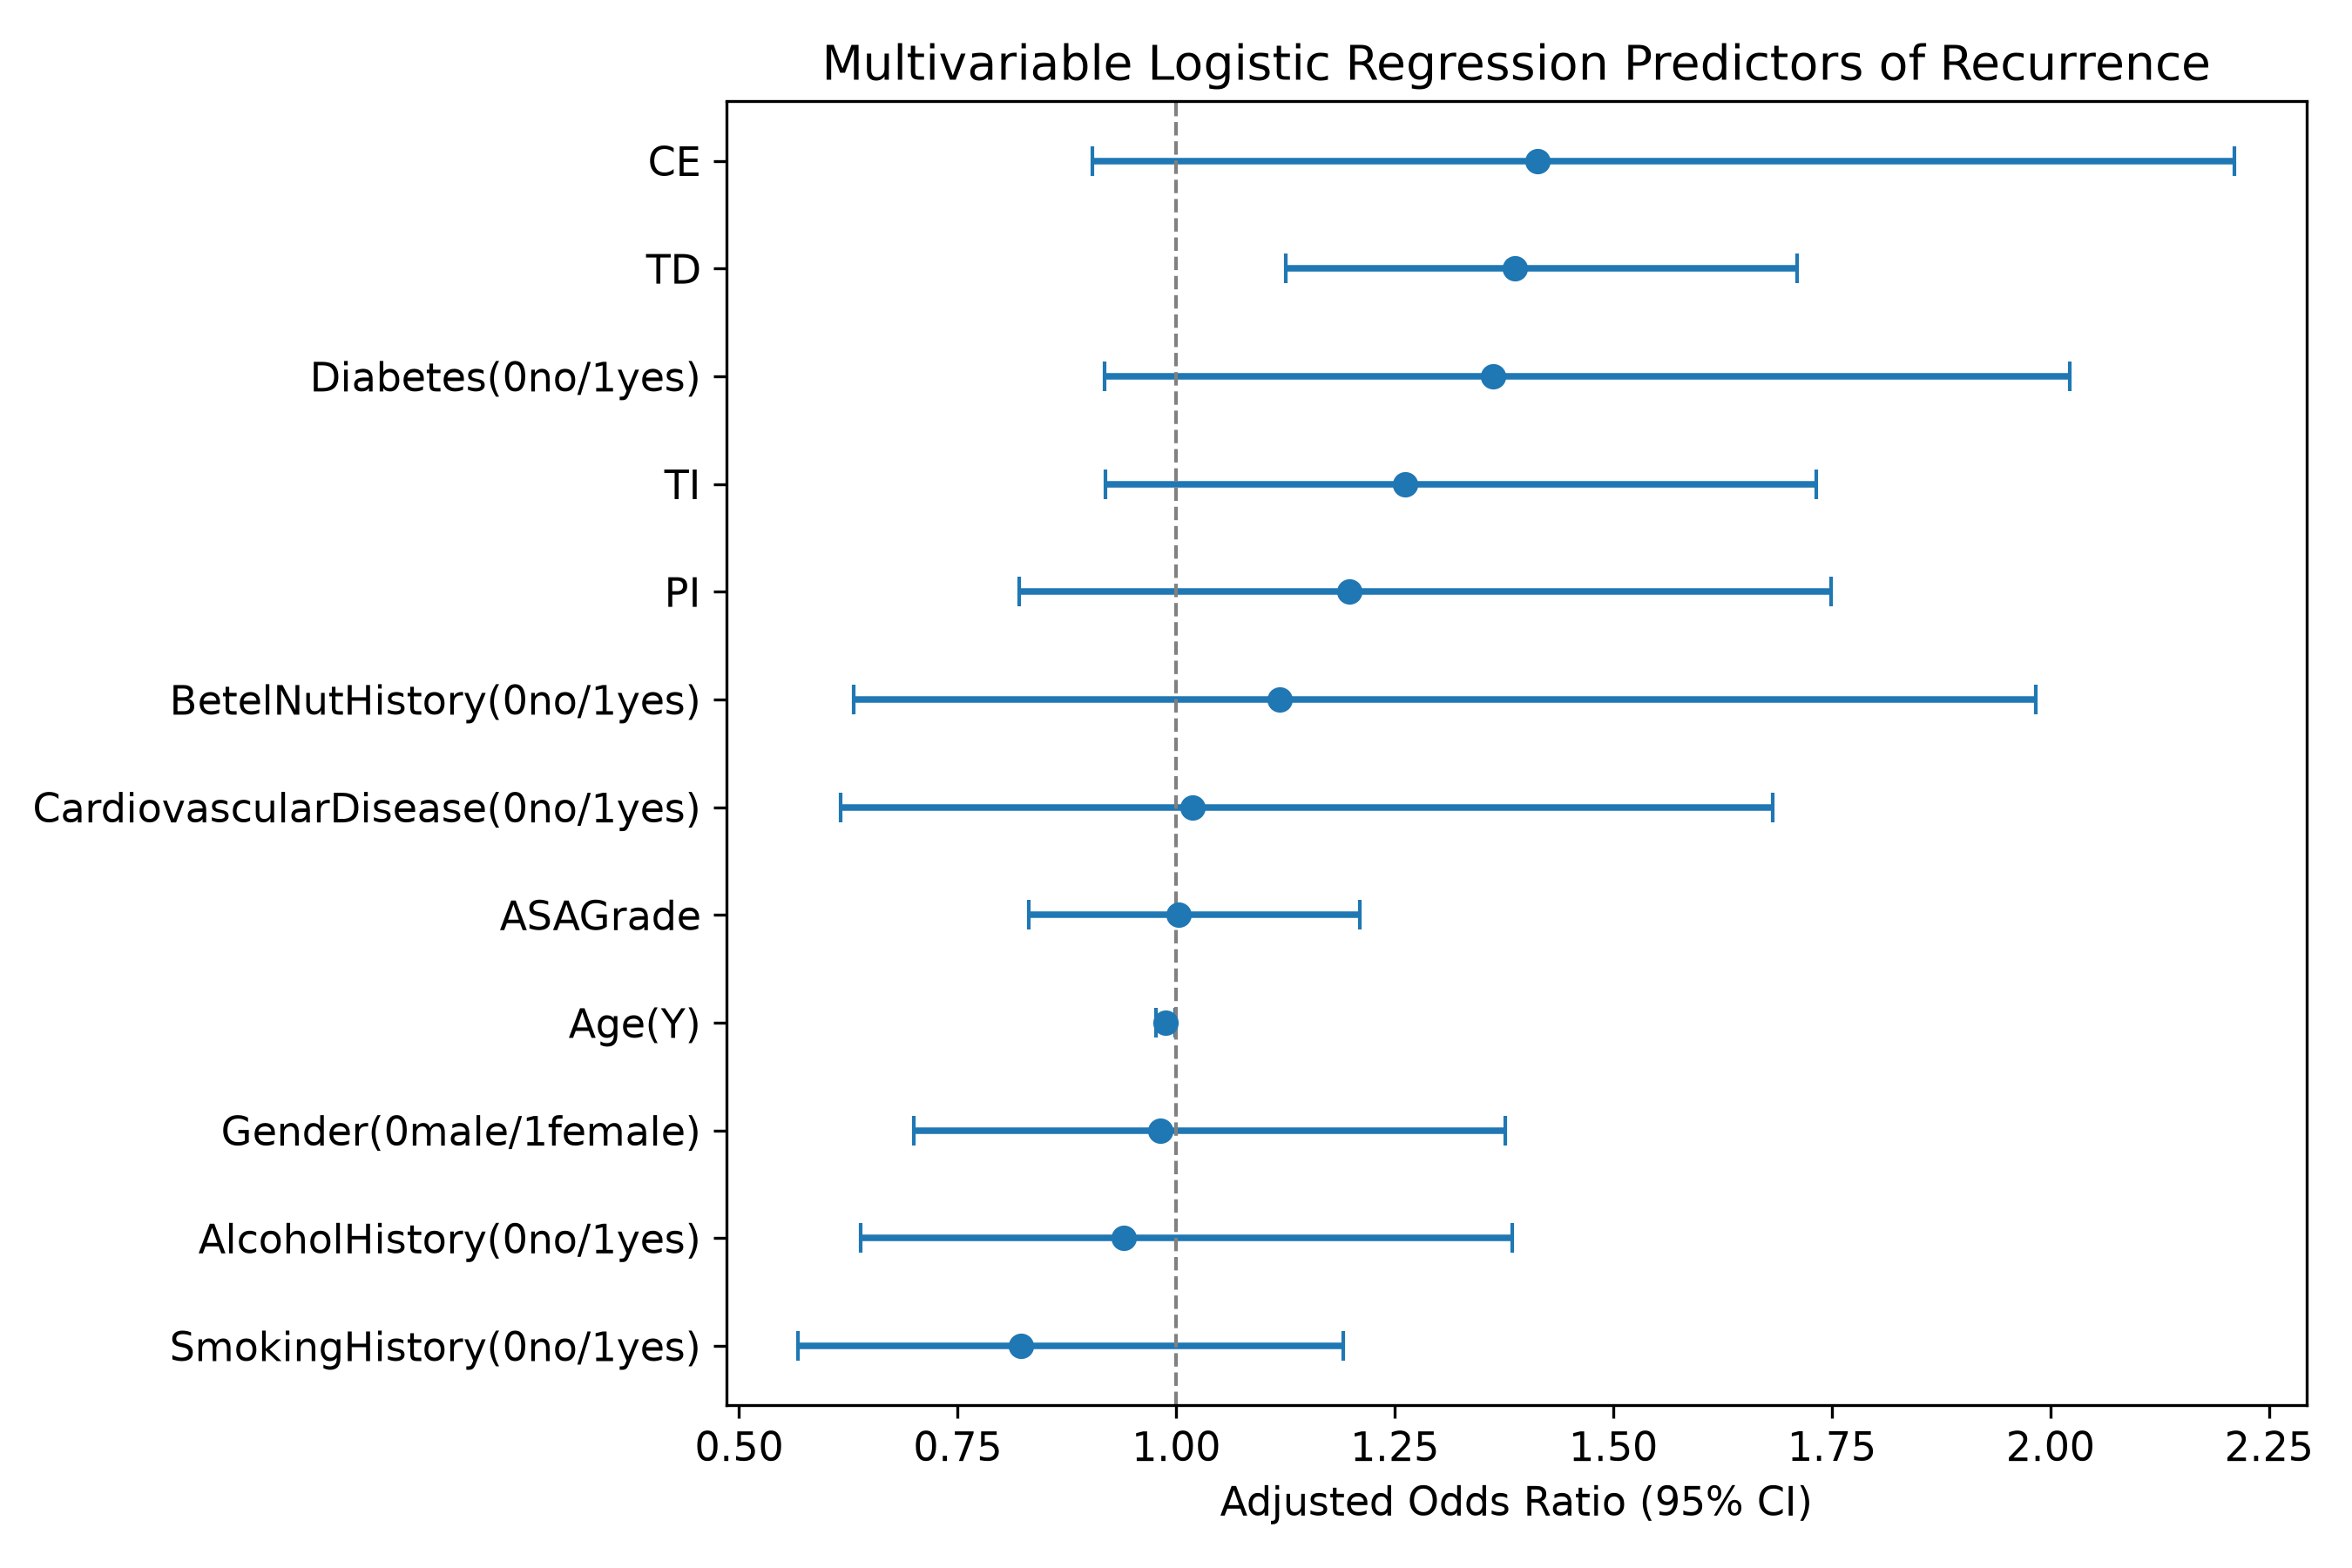
\includegraphics[width=0.80\linewidth]{forest_plot_odds_ratios.png}

\caption{Adjusted odds ratios from the multivariable logistic regression model. Points indicate adjusted odds ratios and horizontal lines indicate 95\% confidence intervals.}

\label{fig:forest}

\end{figure}

The TD odds ratio represents the estimated recurrence-odds change associated with a one-grade worsening in differentiation, under an ordinal linearity assumption. In machine-learning pipelines, TD was one-hot encoded to permit category-specific effects.

\subsection{Model Performance}

Clinical-only models showed weak discrimination (\ROC{} 0.534--0.537). Pathology-only models achieved the highest observed \ROC{}, reaching 0.627 for RF. Adding clinical variables reduced observed \ROC{}, although Combined LR achieved the highest observed \AUPRC{} of 0.429.

\begin{table}[htbp]

\centering

\small

\caption{Held-Out Test Performance ($n=200$; 49 Recurrence Events).}

\label{tab:performance}

\scriptsize
\begin{tabular*}{\linewidth}{@{\extracolsep{\fill}}lcccccc@{}}

\toprule

\textbf{Model} & \textbf{Features} & \textbf{\ROC{}} & \textbf{\AUPRC{}} & \textbf{F1} & \textbf{Recall} & \textbf{\Brier{}} \\

\midrule

LR & Clinical & 0.537 & 0.333 & 0.371 & 0.571 & 0.259 \\

RF & Clinical & 0.534 & 0.334 & 0.415 & 0.551 & 0.244 \\

LR & Pathology & 0.618 & 0.329 & 0.386 & 0.571 & 0.246 \\

RF & Pathology & \textbf{0.627} & 0.406 & 0.400 & \textbf{0.633} & 0.241 \\

LR & Combined & 0.564 & \textbf{0.429} & 0.340 & 0.490 & 0.254 \\

RF & Combined & 0.557 & 0.373 & 0.347 & 0.429 & \textbf{0.239} \\

\bottomrule

\end{tabular*}

\vspace{0.1cm}

\parbox{\linewidth}{\footnotesize The Multi-OSCC authors report an image-based REC benchmark of 0.947 under their own experimental protocol. This result is cited only as dataset context, not as a direct comparator for the tabular models reported here. F1 and recall use a threshold of 0.50.}

\end{table}

\begin{figure}[htbp]

\centering

\begin{subfigure}[b]{0.48\textwidth}

    \centering

    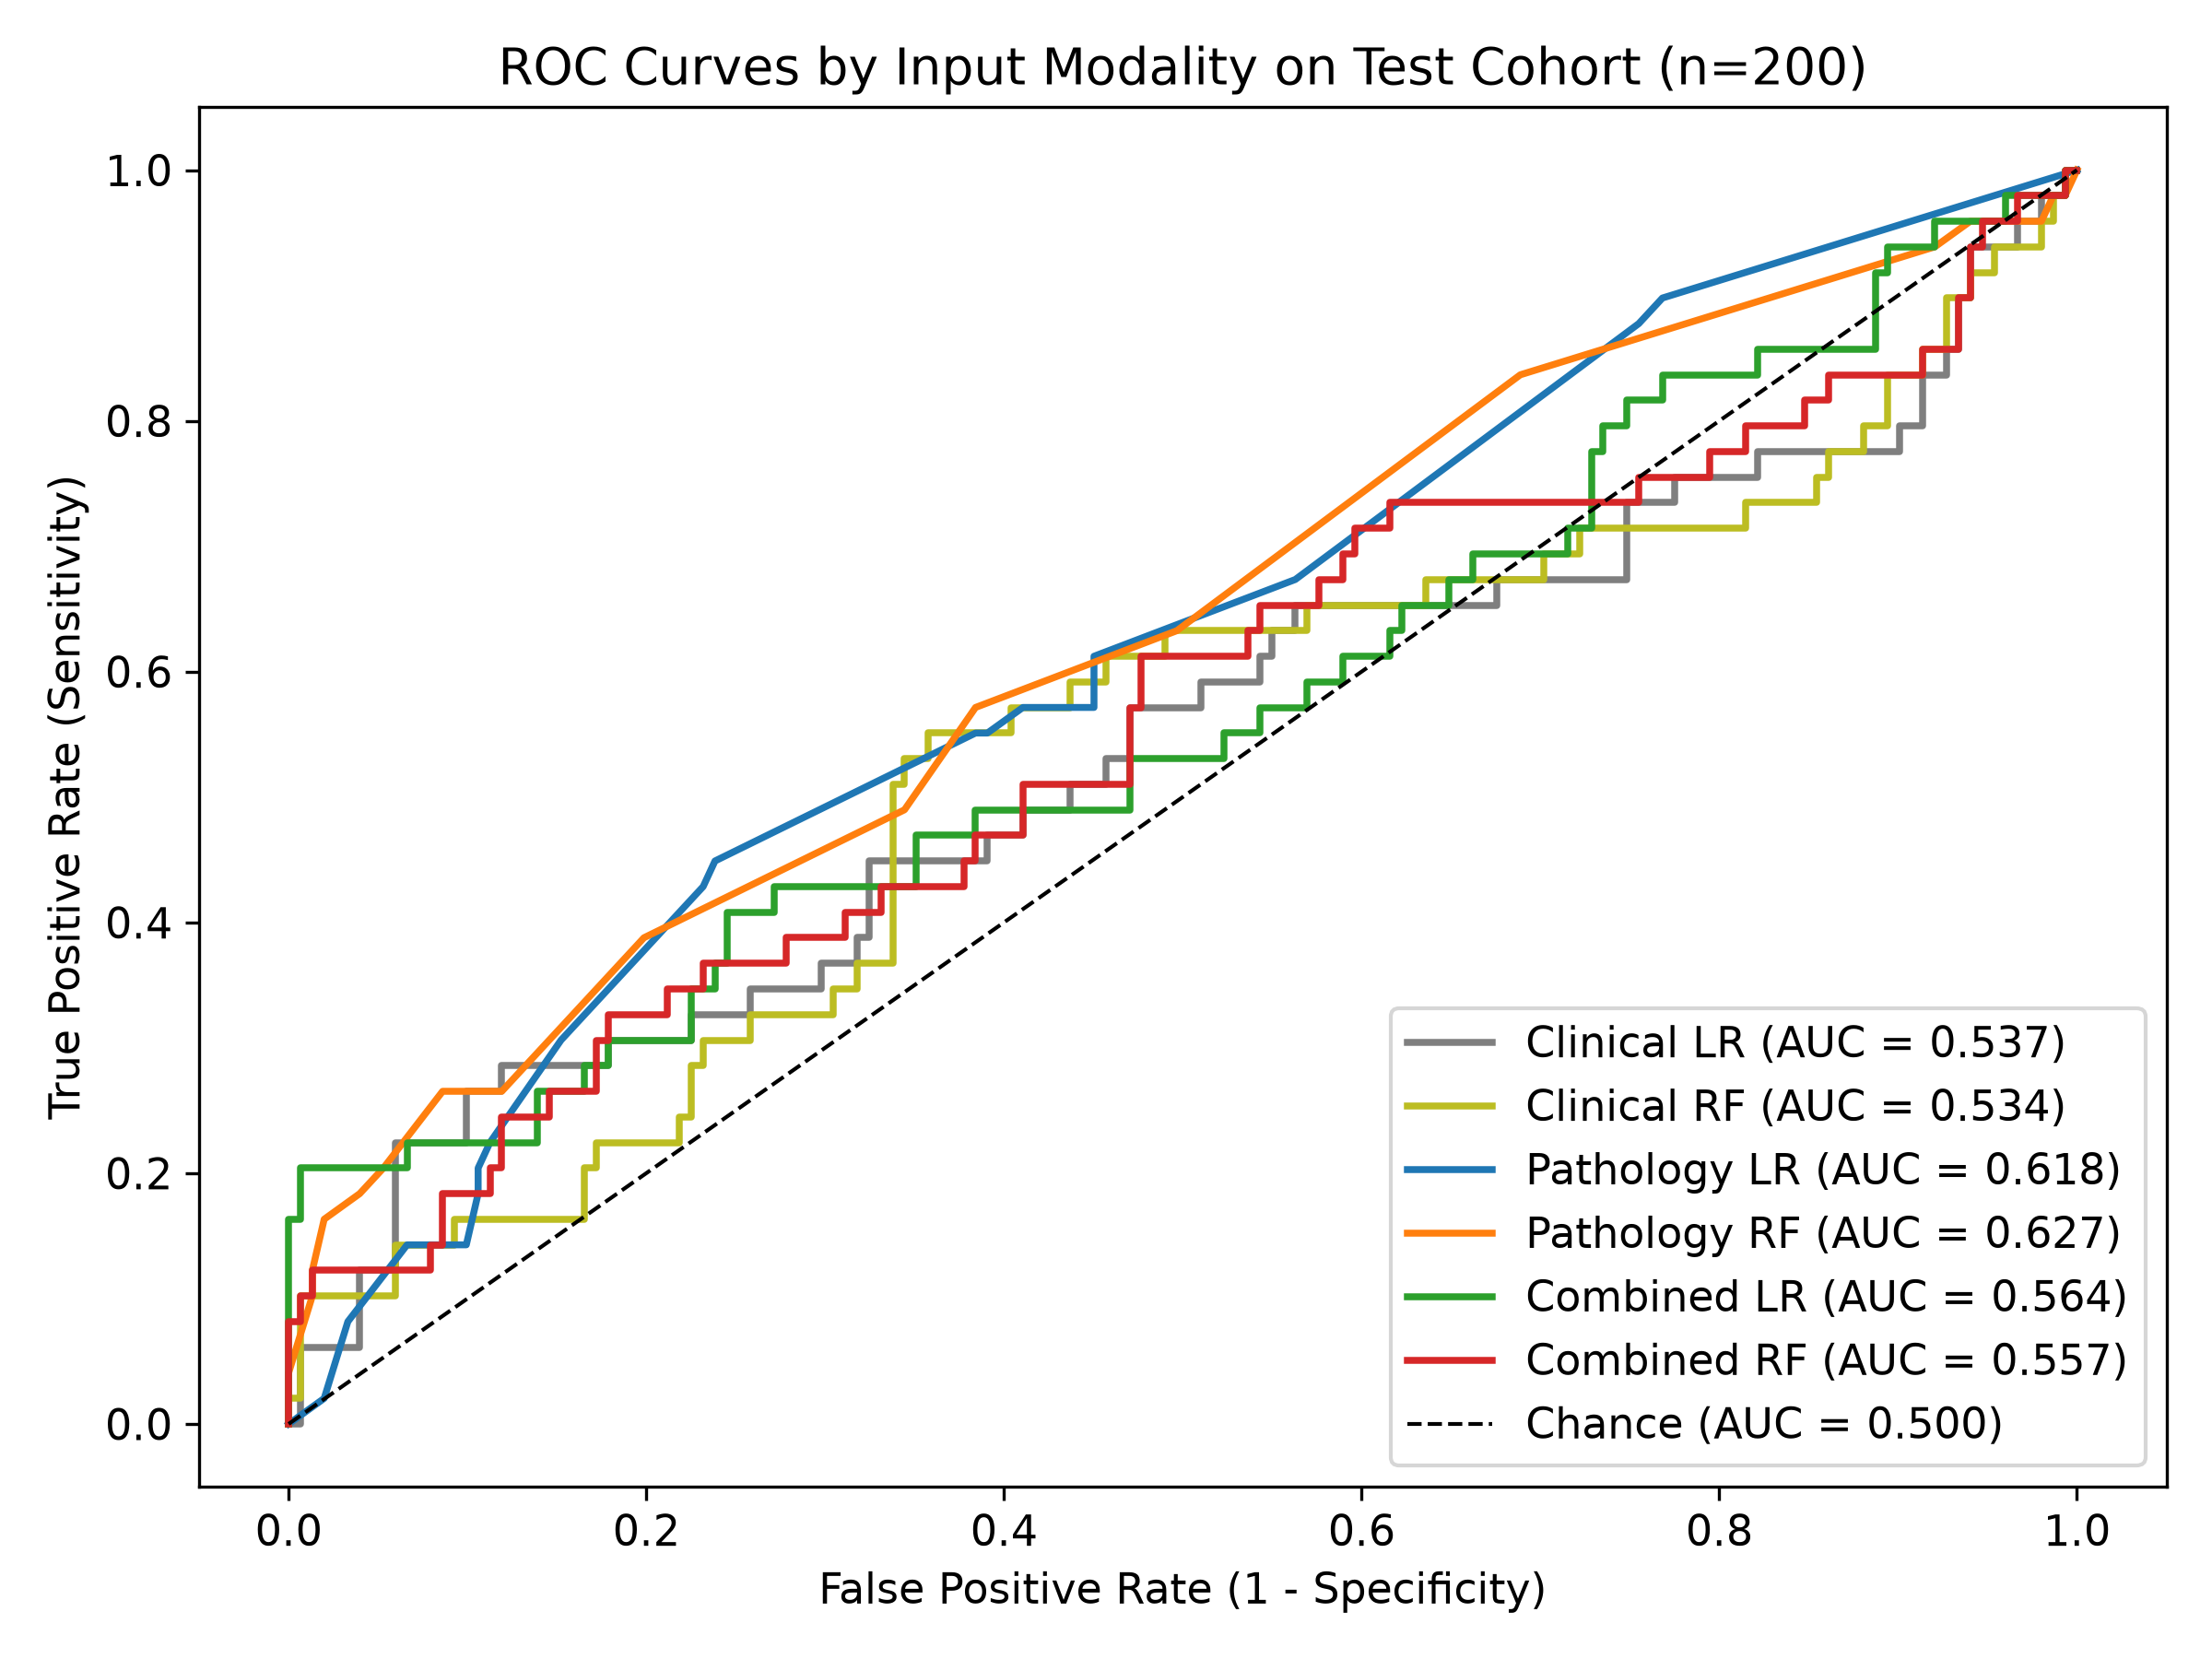
\includegraphics[width=\linewidth]{roc_curves.png}

    \caption{ROC curves.}

    \label{fig:roc}

\end{subfigure}

\hfill

\begin{subfigure}[b]{0.48\textwidth}

    \centering

    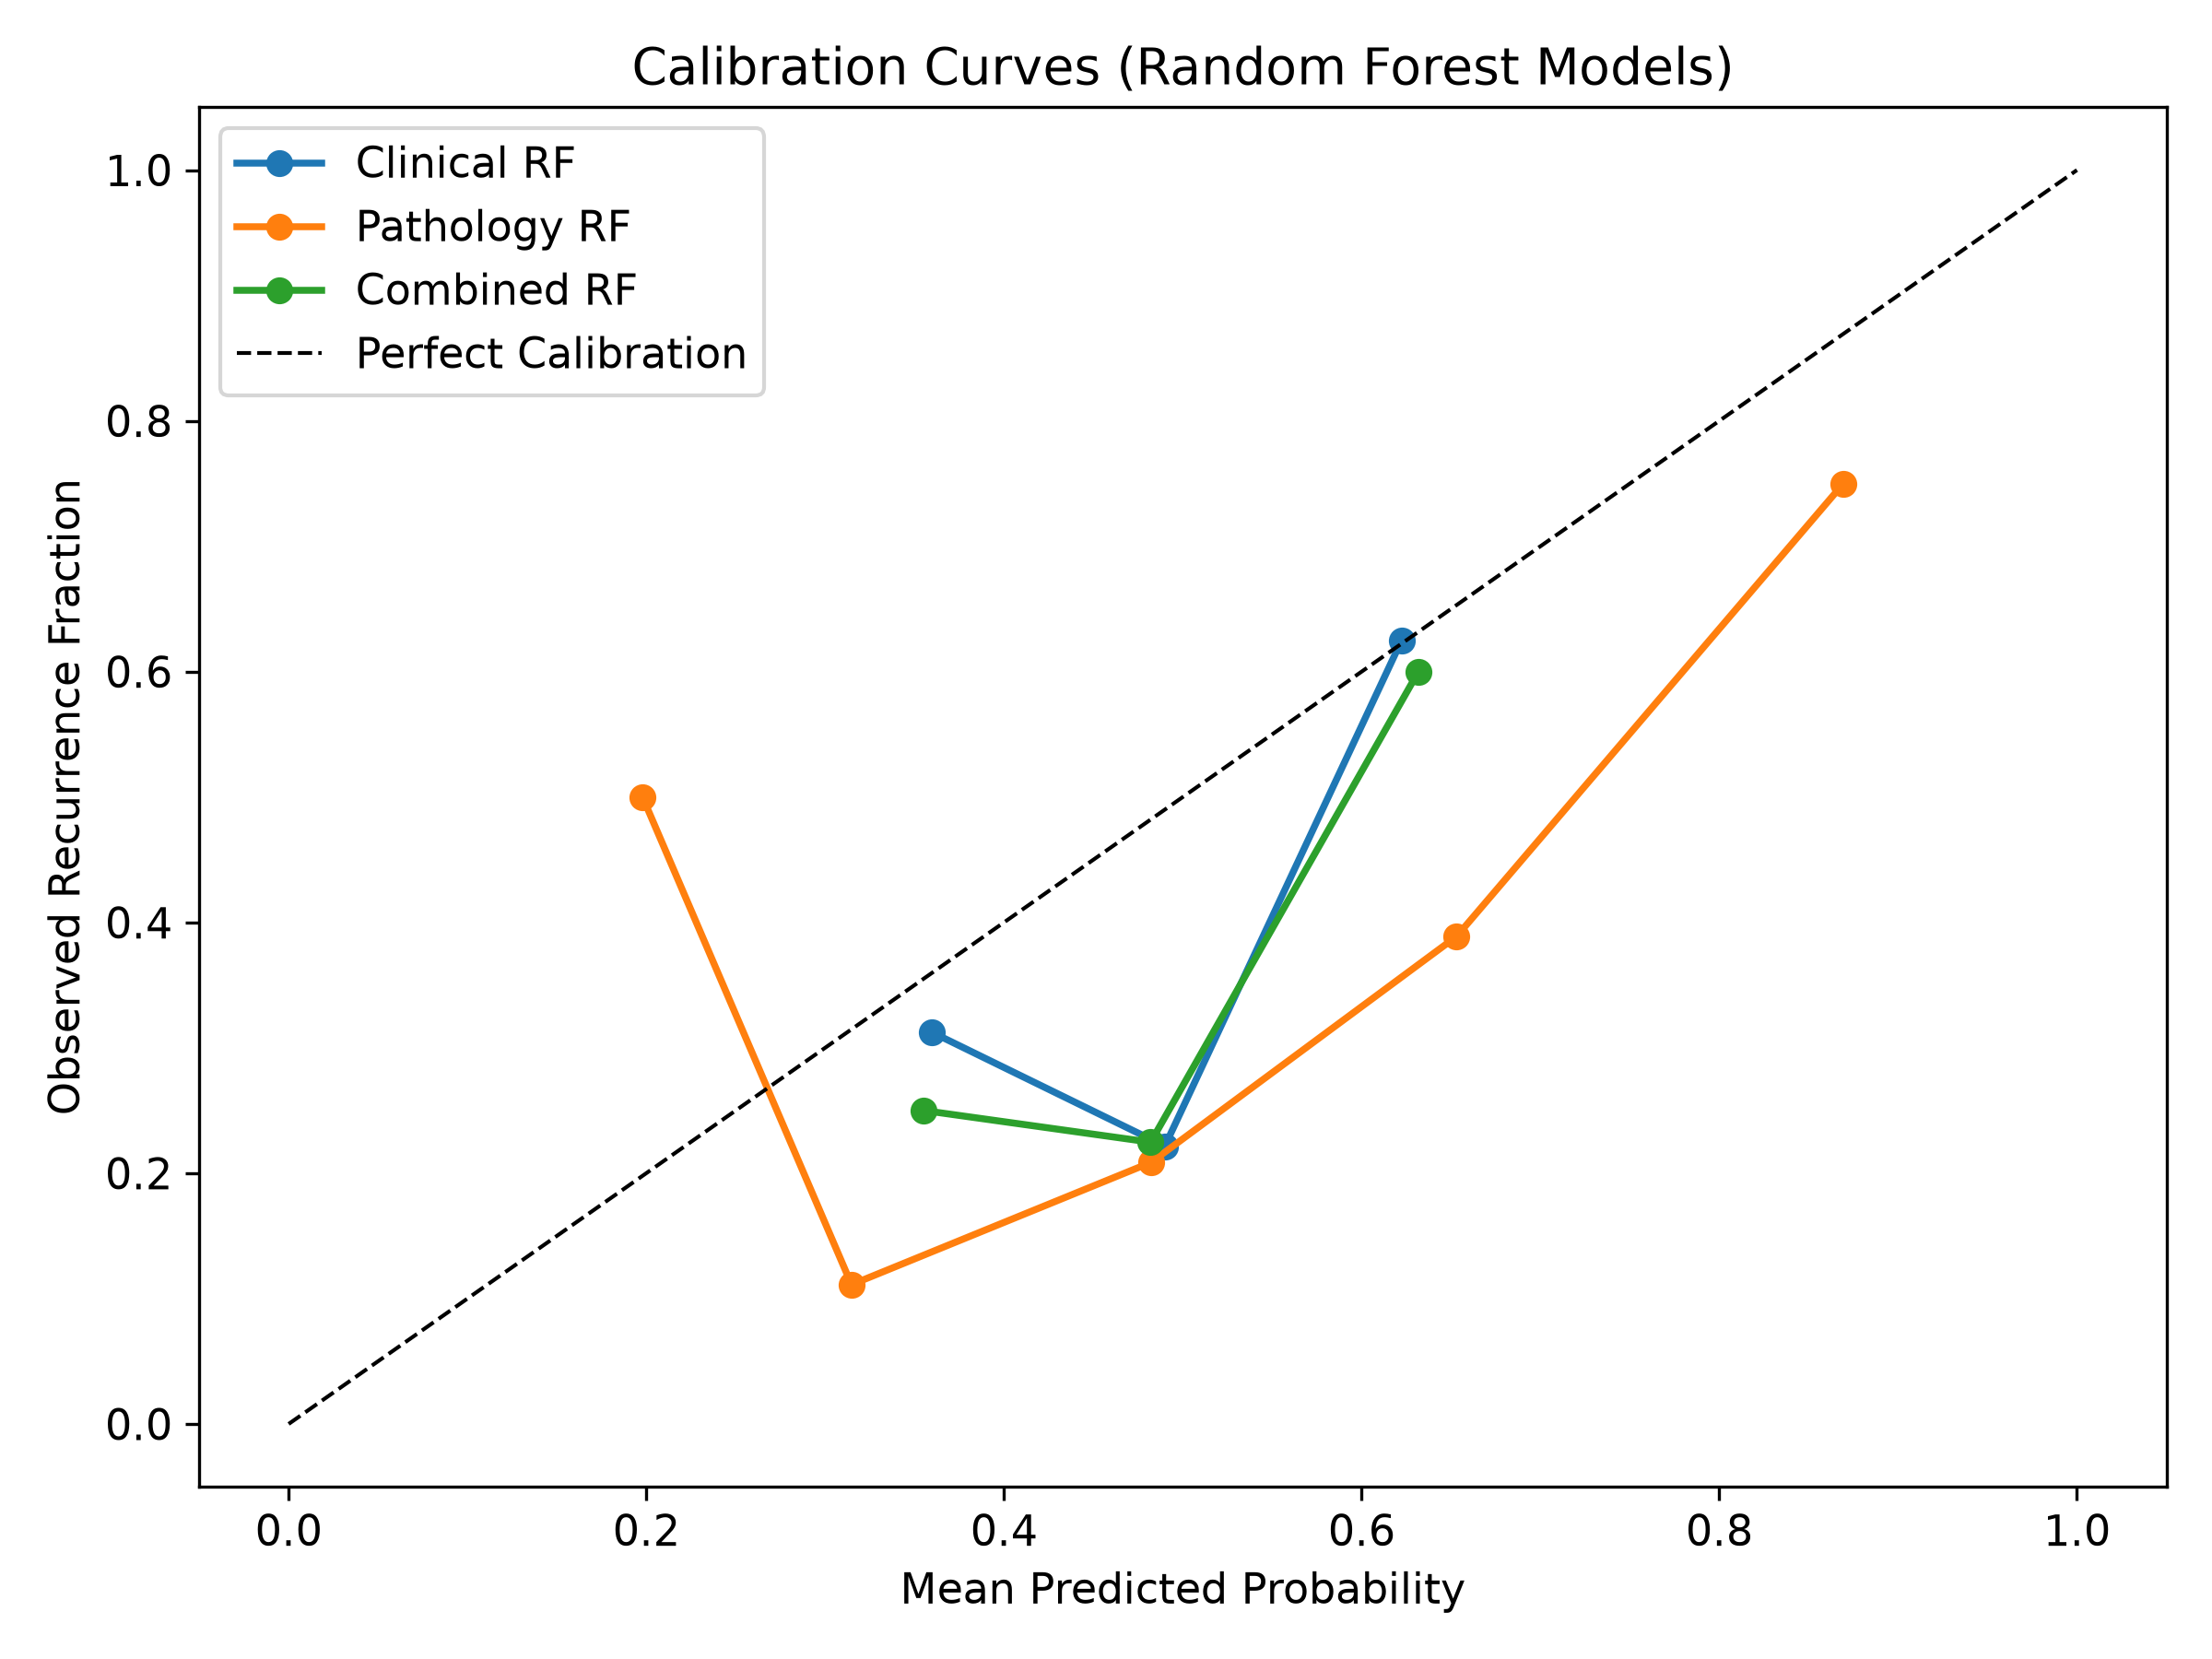
\includegraphics[width=\linewidth]{calibration_curves.png}

    \caption{Random Forest calibration curves.}

    \label{fig:calibration}

\end{subfigure}

\caption{Discrimination and exploratory calibration on the held-out test partition.}

\label{fig:evaluation}

\end{figure}

\subsection{Calibration, Thresholds, and Uncertainty}\label{sec:calibration}

The held-out test prevalence was $49/200=0.245$, giving a prevalence-only \Brier{} benchmark of $p(1-p)=0.184975$. All models had larger \Brier{} scores, indicating greater overall squared probabilistic error than the constant prevalence predictor. The \Brier{} score is not a calibration measure alone and therefore does not by itself establish poor calibration. Calibration intercepts ranged from $-1.21$ to $-1.07$, with the calibration slope fixed at 1 in the corresponding intercept analysis. The negative intercepts indicate systematic upward displacement of predicted recurrence probabilities on the probability scale under this specification. This pattern is consistent with the use of balanced class weights in both LR and RF: the models were trained with recurrence treated as artificially common, which tends to inflate predicted probabilities relative to the true prevalence and can distort threshold-based metrics more than ranking metrics.

At the default threshold of 0.50, Pathology RF identified 31 of 49 recurrence events. A threshold of 0.453203, chosen by maximizing F1 score on the validation partition, identified 41 recurrence events on the test set but resulted in 104 false positives among 151 non-recurrence cases. This illustrates that changing a probability threshold changes the balance between missed recurrences and false alarms; it does not change the underlying ranking ability measured by \ROC{}.

\begin{table}[htbp]

\centering

\small

\caption{Selected Secondary Analyses on the Held-Out Test Cohort.}

\label{tab:secondary}

\scriptsize

\begin{tabularx}{\linewidth}{@{}l l c X@{}}

\toprule

\textbf{Analysis} & \textbf{Model} & \textbf{Result} & \textbf{95\% CI / Detail} \\

\midrule

Bootstrap \ROC{} & Pathology RF & 0.627 & [0.528, 0.724] \\

Bootstrap \AUPRC{} & Pathology RF & 0.406 & [0.286, 0.547] \\

Paired AUC difference & Pathology RF--Combined RF & +0.069 & [$-0.018$, 0.160]; CI includes zero \\

Default threshold & Pathology RF, 0.50 & Recall 0.633 & 31 TP, 75 FP, 76 TN, 18 FN \\

Validation threshold & Pathology RF, 0.453 & Recall 0.837 & 41 TP, 104 FP, 47 TN, 8 FN \\

Seed robustness & Pathology RF & AUC 0.627--0.633 & Seeds 2024, 42, and 123 \\

\bottomrule

\end{tabularx}

\end{table}

Paired bootstrap comparisons did not provide evidence of a statistically significant \ROC{} difference between the Pathology-only and Combined configurations, as the confidence interval for their observed AUC difference included zero. Similar comparisons with the Clinical-only configuration were also not statistically established. The seed analysis produced Pathology RF AUC values from 0.627 to 0.633 across seeds 2024, 42, and 123. This represents limited sensitivity analysis under the same general evaluation framework rather than independent validation.

\section{Discussion}

The results are easiest to interpret as a sequence of scientific questions rather than as a search for a single model. Pathology-derived variables showed stronger observed prognostic signal than the clinical, exposure-history, and comorbidity variables represented in the early information set evaluated here. TD remained associated with recurrence in the adjusted model, whereas smoking, alcohol use, and betel-nut use did not show statistically significant independent associations. This distinction is biologically plausible: exposure variables may contribute primarily to carcinogenesis, while pathological phenotype may more directly reflect invasion and tumor aggressiveness.

Pathology RF achieved the highest observed test-set discrimination (\ROC{} 0.627), although its bootstrap confidence interval was wide and paired comparisons did not establish a statistically significant advantage over competing feature configurations. Adding clinical variables did not improve observed \ROC{} and reduced RF discrimination. This may reflect finite-sample variation, feature redundancy, weak incremental signal, or the expanded one-hot-encoded feature space rather than a causal disadvantage of multimodal models.

Threshold selection illustrates the trade-off between detection and false-positive burden. The validation-selected Pathology RF threshold detected 41 of 49 recurrence events but labelled 104 non-recurrence patients as high risk. Such an operating point may be relevant only if a high-risk classification leads to low-harm follow-up, such as additional examination or imaging, rather than immediate invasive intervention.

Whole-slide images may contain spatial and morphological information unavailable in coarse categorical pathology variables, including tumor--stroma architecture, cellular heterogeneity, inflammatory infiltration, and invasive growth patterns \cite{almangush_staging_2020}. The published Multi-OSCC image benchmark reported higher image-based performance \cite{guan2026multi}; however, direct comparison is inappropriate unless population, outcome definition, partitioning, slide selection, and validation protocol are shown to be equivalent.

\subsection{Limitations}

The study has several limitations:

\begin{itemize}

    \item It is observational and evaluates association and prediction rather than causality.

    \item The held-out test cohort contained only 49 recurrence events, limiting precision and producing wide confidence intervals.

    \item All tabular models showed systematic probability overestimation under the calibration-intercept analysis, and their \Brier{} scores were above the prevalence-only benchmark; no recalibration was applied.

    \item HPV status was excluded because 22.4\% of observations were missing.

    \item The dataset paper reports at least two years of post-operative follow-up for inclusion, but this analysis did not independently reconstruct follow-up completeness for every released record; endpoint ascertainment is therefore inherited from the dataset and was not independently audited.

    \item The pathology representation was limited to four categorical variables and may not capture information visible in the underlying histopathology images.

    \item Multiple univariate association tests were exploratory and were not adjusted for multiplicity; their p-values should therefore be interpreted as screening evidence rather than as a set of independent confirmatory tests.

    \item Bootstrap intervals were conditional on the fitted models and held-out predictions; they do not incorporate uncertainty from alternative partitions or model-development choices.

    \item External validation is required before clinical deployment.

\end{itemize}

\section{Conclusion}

In this retrospective OSCC recurrence analysis, pathology-derived variables provided stronger observed ranking information than the clinical, lifestyle, and comorbidity variables evaluated in the held-out cohort. Because TD, TI, CE, and PI are derived from surgical specimens, these results should not be described as pre-treatment prediction. Tumor Differentiation remained associated with recurrence in adjusted logistic regression, and Pathology RF achieved the highest observed tabular \ROC{}.

However, discrimination was moderate, pairwise model differences were not statistically established, and the predicted probabilities were not well aligned with the prevalence scale under the calibration analysis. A validation-selected high-recall threshold substantially increased false-positive classifications, illustrating the trade-off between missed recurrences and additional follow-up workload. These models should therefore be interpreted as exploratory tools for risk stratification rather than clinically deployable recurrence predictors. External validation, recalibration, standardized follow-up definitions, and prospective evaluation of clinically meaningful surveillance strategies are necessary.

\bibliographystyle{unsrt}
\bibliography{refs}

\end{document}